\documentclass[aspectratio=169, hideothersubsections]{beamer}
%\documentclass{beamer}
%\documentclass[aspectratio=1610]{beamer}
\usepackage{listings}
\usepackage{graphicx}
\usepackage{tikz}
\usetheme{Berkeley}
\usefonttheme{structuresmallcapsserif}
\usecolortheme{owl}
%\usepackage{xcolor}
%\usepackage{darkmode}
%\enabledarkmode
%\usecolortheme{albatross}
%\usecolortheme{spruce}
\usepackage{minted}
\usepackage{comment}
\usepackage{animate}  


\setbeamertemplate{page number in head/foot}[totalframenumber]
\setbeamertemplate{navigation symbols}{\footnotesize\usebeamertemplate{page number in head/foot}}
\setbeamercolor{title}{fg = OwlRed}
\setbeamercolor{author}{fg = OwlBlue}
%\setbeamercolor{frametitle}{fg=white}
%\setbeamercolor{background canvas}{bg=black}
%\setbeamercolor{normal text}{fg=white}

%--------------------------------------
%REPLACE IMAGE.JPG WITH LOGO OF ORGANISATION
\logo{\begin{tikzpicture}
\node[inner sep=0pt] at (0,0) {
\includegraphics[height=1cm]{SODS Logo.png}};
\end{tikzpicture}}
%--------------------------------------

\title{BSDS-206 : Text Analytics}
\subtitle{Course Instructor - Dr. Aashima Bangia}
\author[Gauri Sharan]{Gauri Sharan - BSc Data Science, Semester 4}
\date{June 11, 2024}

\begin{document}
\frame{\titlepage}

\begin{frame}{Table of contents}
    \tableofcontents[hideallsubsections]
\end{frame}

%Unit 1
\section{Text Processing and Mining}

\subsection{NLP Concepts}

\subsection{Data Handling}

\begin{frame}[fragile]{Extracting Data}
\begin{block}{Extracting Data}
    Extracting data from various sources such as PDFs, Word files, JSON, HTML, etc.
  \end{block}
\rule{\textwidth}{1pt}
\scriptsize
\begin{minted}{python}
import re
text = "Hello, World!"
pattern = r'\w+'
matches = re.findall(pattern, text)
print(matches)
\end{minted}
\rule{\textwidth}{1pt}
\end{frame}

\begin{frame}[fragile]{Collecting Data}
\begin{block}{Collecting Data}
    Collecting data from various sources using libraries and tools.
  \end{block}
\rule{\textwidth}{1pt}
\scriptsize
\begin{minted}{python}
import json
with open('data.json') as f:
    data = json.load(f)
print(data)
\end{minted}
\rule{\textwidth}{1pt}
\end{frame}

\begin{frame}[fragile]{Parsing Data}
\begin{block}{Parsing}
    Reading and interpreting data using regular expressions.
  \end{block}
\rule{\textwidth}{1pt}
\scriptsize
\begin{minted}{python}
import re
text = "Hello, World!"
pattern = r'\w+'
matches = re.findall(pattern, text)
print(matches)
\end{minted}
\rule{\textwidth}{1pt}
\end{frame}

\begin{frame}[fragile]{Structuring Data}
\begin{block}{Structuring Data}
    Handling strings, scraping data from the web, and exploring and preprocessing text data.
\end{block}
\rule{\textwidth}{1pt}
\scriptsize
\begin{minted}{python}
import pandas as pd
df = pd.DataFrame({
    'Name': ['John', 'Mary', 'Jane'],
    'Age': [25, 30, 35]
})
print(df)
\end{minted}
\rule{\textwidth}{1pt}
\end{frame}

\subsection{Preprocessing}
\begin{frame}
\frametitle{Exploring and Preprocessing Text Data}
NLP Python Libraries:
\begin{description}
\setbeamercolor{item}{fg = OwlBlue}
    \item[NLTK] Natural Language Toolkit: A comprehensive library for NLP tasks such as tokenization, stemming, tagging, parsing, and semantic reasoning. It is widely used for text preprocessing and machine learning tasks.
    \item[spaCy] A modern NLP library that focuses on production-ready models for NLP tasks such as tokenization, entity recognition, and language modeling. It is known for its high-performance and ease of use.
    \item[Gensim] A library for topic modeling and document similarity analysis. It is particularly useful for processing large volumes of text data and extracting insights from it. 
\end{description}
\end{frame}


\begin{frame}[fragile]{Python Code Example - Exploring and Preprocessing Data}
\rule{\textwidth}{1pt}
\scriptsize
\begin{minted}{python}
import re
import requests
from bs4 import BeautifulSoup

# Scraping example
url = 'http://example.com'
response = requests.get(url)
soup = BeautifulSoup(response.text, 'html.parser')
text = soup.get_text()

# Regular expression example
pattern = re.compile(r'\b[A-Za-z]+\b')
matches = pattern.findall(text)
print(matches)
\end{minted}
\rule{\textwidth}{1pt}
\end{frame}


%unit 2
\section{Raw Textual Data to Features}

\subsection{Raw Text to Features}

\begin{frame}[fragile]{Converting Text Data to Lowercase}
  \begin{block}{Why Lowercase?}
    Lowercase text is easier to process and compare.
  \end{block}
\rule{\textwidth}{1pt}
\scriptsize
\begin{minted}{python}
import string
text = "Hello, World!"
text = text.lower()
print(text)
\end{minted}
\rule{\textwidth}{1pt}
\end{frame}

\begin{frame}[fragile]{Removing Punctuation}
  \begin{block}{Why Remove Punctuation?}
    Punctuation can affect the accuracy of text processing.
  \end{block}
\rule{\textwidth}{1pt}
\scriptsize
\begin{minted}{python}
import string
text = "Hello, World!"
text = text.translate(str.maketrans('', '', string.punctuation))
print(text)
\end{minted}
\rule{\textwidth}{1pt}
\end{frame}

\begin{frame}[fragile]{Removing Stop Words}
  \begin{block}{Why Remove Stop Words?}
    Stop words are common words that do not carry much meaning.
  \end{block}
\rule{\textwidth}{1pt}
\scriptsize
\begin{minted}{python}
import nltk
from nltk.corpus import stopwords
stop_words = set(stopwords.words('english'))
text = "Hello, World!"
words = text.split()
filtered_words = [word for word in words if word not in stop_words]
print(filtered_words)
\end{minted}
\rule{\textwidth}{1pt}
\end{frame}

\begin{frame}[fragile]{Standardizing Text}
  \begin{block}{Tokenization}
    Breaking text into individual words or tokens.
  \end{block}
  \begin{block}{Stemming}
    Reducing words to their base form.
  \end{block}
  \begin{block}{Lemmatizing}
    Reducing words to their base form using a dictionary.
  \end{block}
\rule{\textwidth}{1pt}
\scriptsize
\begin{minted}{python}
import nltk
from nltk.stem import WordNetLemmatizer
lemmatizer = WordNetLemmatizer()
text = "running"
print(lemmatizer.lemmatize(text))
\end{minted}
\rule{\textwidth}{1pt}
\end{frame}

\subsection{Text Processing Pipeline}
\begin{frame}{Building a Text Processing Pipeline - Converting Text to Features}
\begin{block}{Why Pipeline?}
    Pipelines help to streamline text processing tasks.
\end{block}
  \begin{itemize}
    \item One-hot encoding
    \item Count Vectorizing
    \item TF-IDF
    \item Generating N-grams, Co-occurrence Matrix, Hash Vectorizing
    \item Implementing Word Embeddings
  \end{itemize}
\end{frame}

\begin{frame}[fragile]{Python Code Example - Pipeline}
\rule{\textwidth}{1pt}
\scriptsize
\begin{minted}{python}
from sklearn.feature_extraction.text import CountVectorizer, TfidfVectorizer

# Example text
texts = ["This is a sentence.", "This is another sentence."]

# Count Vectorizer
count_vectorizer = CountVectorizer()
X_count = count_vectorizer.fit_transform(texts)
print(X_count.toarray())

# TF-IDF Vectorizer
tfidf_vectorizer = TfidfVectorizer()
X_tfidf = tfidf_vectorizer.fit_transform(texts)
print(X_tfidf.toarray())
\end{minted}
\rule{\textwidth}{1pt}
\end{frame}

%unit 3
\section{Advanced Processes}

\subsection{POS Tagging}

\begin{frame}[fragile]{POS Tagging}
  \begin{block}{What is POS Tagging?}
    Part-of-speech tagging is the process of identifying the part of speech of each word in a sentence.
  \end{block}
  \begin{block}{Why POS Tagging?}
    POS tagging is useful for tasks such as sentiment analysis and named entity recognition.
  \end{block}
\rule{\textwidth}{1pt}
\scriptsize
\begin{minted}{python}
import nltk
from nltk import pos_tag
text = "Hello, World!"
tokens = word_tokenize(text)
pos_tags = pos_tag(tokens)
print(pos_tags)
\end{minted}
\rule{\textwidth}{1pt}
\end{frame}

\subsection{Topic Modeling}

\begin{frame}
  \frametitle{Topic Modeling}
  \begin{block}{What is Topic Modeling?}
    Topic modeling is the process of identifying topics or themes in a large corpus of text.
  \end{block}
  \begin{block}{Why Topic Modeling?}
    Topic modeling is useful for tasks such as text classification and clustering.
  \end{block}
  \begin{block}{Topic Modelling Techniques}
      \begin{itemize}
        \item Latent Dirichlet Allocation (LDA)
        \item Non-Negative Matrix Factorization (NMF)
        \item Latent Semantic Analysis (LSA)
        \item Parallel Latent Dirichlet Allocation (PLDA)
      \end{itemize}
  \end{block}
\end{frame}

\begin{frame}[fragile]{Python code example - Topic Modelling}
\rule{\textwidth}{1pt}
\scriptsize
\begin{minted}{python}
import nltk
from nltk.tokenize import word_tokenize
from nltk.corpus import stopwords
from nltk.stem import WordNetLemmatizer
from sklearn.feature_extraction.text import TfidfVectorizer
from sklearn.decomposition import LatentDirichletAllocation
def topic_modeling(text):
    tokens = word_tokenize(text)
    stop_words = set(stopwords.words('english'))
    filtered_tokens = [token for token in tokens if token not in stop_words]
    lemmatizer = WordNetLemmatizer()
    lemmatized_tokens = [lemmatizer.lemmatize(token) for token in filtered_tokens]
    vectorizer = TfidfVectorizer()
    tfidf = vectorizer.fit_transform(lemmatized_tokens)
    lda = LatentDirichletAllocation(n_components=2)
    topics = lda.fit_transform(tfidf)
    return topics

text = "Hello, World!" ; topics = topic_modeling(text)
print(topics)
\end{minted}
\rule{\textwidth}{1pt}
\end{frame}

%unit 4
\section{Word Embeddings and more}

\subsection{Word Embeddings}

\begin{frame}
  \frametitle{Word Embeddings}
  \begin{block}{What are Word Embeddings?}
    Word embeddings are dense vector representations of words.
  \end{block}
  \begin{block}{Why Word Embeddings?}
    Word embeddings are useful for tasks such as text classification and clustering.
  \end{block}
\begin{block}{Word Embedding Techniques}
    \begin{itemize}
    \item Vectorizing, Continuous Bag of Words (CBoW), N-Gram, Word2Vec
    \item Training a Word Embedding through Skip-Grams, CBoW
    \item Global Vectors for Word Representations (GloVe)
    \item Using trained Word Embeddings with LSTMs
    \item Paragraph2Vec: Distributed Memory of Paragraph Vectors (PV-DM)
  \end{itemize}
\end{block}
\end{frame}

\begin{frame}[fragile]{Python Code Example - Word Embedding}
\rule{\textwidth}{1pt}
\scriptsize
\begin{minted}{python}
import numpy as np
from sklearn.preprocessing import Normalizer

def word_embeddings(word):
    # Define word embeddings
    word_embeddings = {
        'hello': np.array([1, 2, 3]),
        'world': np.array([4, 5, 6])
    }
    return word_embeddings.get(word, np.zeros(3))

word = "hello"
embedding = word_embeddings(word)
print(embedding)
\end{minted}
\rule{\textwidth}{1pt}
\end{frame}

\begin{frame}[fragile]{Python Code Example - Word2Vec}
\rule{\textwidth}{1pt}
\scriptsize
\begin{minted}{python}
from gensim.models import Word2Vec

# Example sentences
sentences = [["This", "is", "a", "sentence"], ["This", "is", "another", "sentence"]]

# Train Word2Vec model
model = Word2Vec(sentences, vector_size=100, window=5, min_count=1, workers=4)
print(model.wv['sentence'])
\end{minted}
\rule{\textwidth}{1pt}
\end{frame}

\subsection{Text Generation}

\begin{frame}
  \frametitle{Text Generation}
  \begin{block}{What is Text Generation?}
    Text generation is the process of generating new text based on a given input.
  \end{block}
  \begin{block}{Why Text Generation?}
    Text generation is useful for tasks such as chatbots and language translation.
  \end{block}
\begin{block}{Methods:}
\begin{itemize}
    \item Text Generation with LSTMs
    \item Creating NER tagging
    \item Sequence-to-sequence Models (Seq2Seq)
  \end{itemize}
\end{block}
\end{frame}

\begin{frame}[fragile]{Python Code Example 1 - Text Generation}
\rule{\textwidth}{1pt}
\scriptsize
\begin{minted}{python}
import numpy as np
from sklearn.preprocessing import Normalizer

def text_generation(input_text):
    # Define a simple text generation model
    model = {
        'hello': 'world',
        'world': 'hello'
    }
    return model.get(input_text, 'Unknown')

input_text = "hello"
output_text = text_generation(input_text)
print(output_text)
\end{minted}
\rule{\textwidth}{1pt}
\end{frame}

\begin{frame}[fragile]{Python Code Example 2 - Text Generation}
\rule{\textwidth}{1pt}
\scriptsize
\begin{minted}{python}
from keras.models import Sequential
from keras.layers import LSTM, Dense

model = Sequential()
model.add(LSTM(50, return_sequences=True, input_shape=(100, 1)))
model.add(LSTM(50))
model.add(Dense(1))
model.compile(optimizer='adam', loss='mse')

print(model.summary())
\end{minted}
\rule{\textwidth}{1pt}
\end{frame}


\subsection{Machine Translation}

\begin{frame}[fragile]{Machine Translation}
  \begin{block}{What is Machine Translation?}
    Machine translation is the process of translating text from one language to another.
  \end{block}
  \begin{block}{Why Machine Translation?}
    Machine translation is useful for tasks such as language translation and localization.
  \end{block}
\end{frame}

\begin{frame}[fragile]{Python Code Example - Machine Tanslation}
\rule{\textwidth}{1pt}
\scriptsize
\begin{minted}{python}
import numpy as np
from sklearn.preprocessing import Normalizer

def machine_translation(input_text):
    # Define a simple machine translation model
    model = {
        'hello': 'bonjour',
        'world': 'monde'
    }
    return model.get(input_text, 'Unknown')

input_text = "hello"
output_text = machine_translation(input_text)
print(output_text)
\end{minted}
\rule{\textwidth}{1pt}
\end{frame}

%unit 5
\section{Neural Networks}

\subsection{Understanding Activation Functions in Neural Networks}
\begin{frame}
    \frametitle{Understanding Activation Functions in Neural Networks}
    \begin{block}{Definition}
        Activation functions introduce non-linearity into the neural network.
    \end{block}
    \begin{block}{Common Activation Functions}
        \begin{itemize}
            \item Sigmoid
            \item ReLU (Rectified Linear Unit)
            \item Tanh (Hyperbolic Tangent)
        \end{itemize}
    \end{block}
\end{frame}

\begin{frame}{Activation Functions Graphs}
\begin{figure}
  \centering
  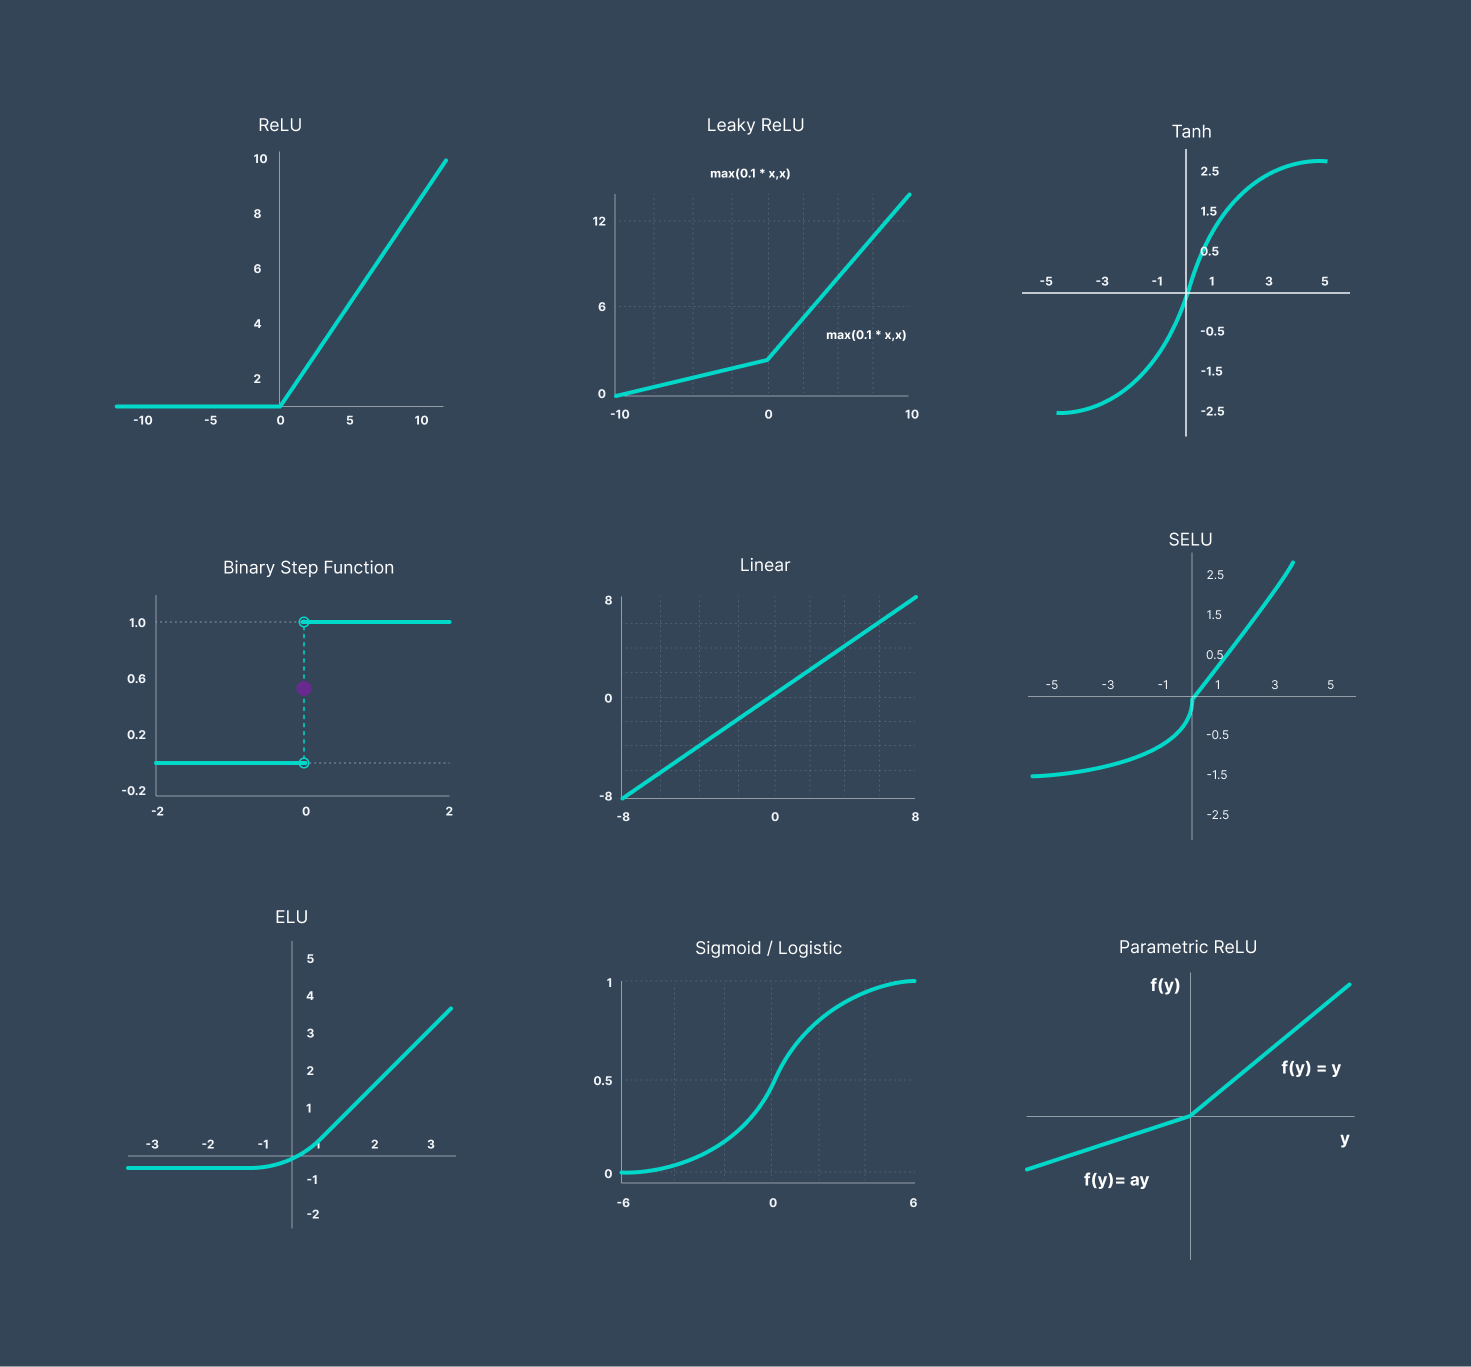
\includegraphics[width=0.4\textwidth]{pic.png}
  \label{fig:example}
  \caption{Activation Functions Graphs}
\end{figure}
\end{frame}

\subsection{Loss Function}
\begin{frame}
    \frametitle{Loss Function}
    \begin{block}{Definition}
        The loss function measures the difference between the predicted output and the actual output.
    \end{block}
    \begin{block}{Common Loss Functions}
        \begin{itemize}
            \item Mean Squared Error (MSE)
            \item Cross-Entropy
        \end{itemize}
    \end{block}
\end{frame}

\subsection{Perceptron:- Single Layered and Multiple Layered}
\begin{frame}
    \frametitle{Perceptron:- Single Layered and Multiple Layered}
    \begin{block}{Single Layer Perceptron}
        A single layer neural network with a linear activation function.
    \end{block}
    \begin{block}{Multi-Layer Perceptron}
        A neural network with multiple layers, allowing for more complex representations.
    \end{block}
\end{frame}

\subsection{Building a Single Neuron Neural Network from Scratch in Python}
\begin{frame}[fragile]{Building a Single Neuron Neural Network from Scratch in Python}
\rule{\textwidth}{1pt}
\scriptsize
\begin{minted}{python}
class Neuron:
    def __init__(self, inputs, bias):
        self.weights = [random.random() for _ in range(inputs)]
        self.bias = bias

    def forward(self, inputs):
        output = sum([x * y for x, y in zip(inputs, self.weights)]) + self.bias
        return self.sigmoid(output)

    def sigmoid(self, x):
        return 1 / (1 + math.exp(-x))

neuron = Neuron(2, 1)
inputs = [0, 0]
output = neuron.forward(inputs)
print(output)
\end{minted}
\rule{\textwidth}{1pt}
\end{frame}

\subsection{Practical Implementation of Neural Network Training in Python}
\begin{frame}[fragile]{Practical Implementation of Neural Network Training in Python}
\rule{\textwidth}{1pt}
\scriptsize
\begin{minted}{python}
import numpy as np
# Define the neural network
class NeuralNetwork:
    def __init__(self, inputs, hidden, outputs):
        self.weights1 = np.random.rand(inputs, hidden)
        self.weights2 = np.random.rand(hidden, outputs)

    def forward(self, inputs):
        hidden_layer = np.maximum(np.dot(inputs, self.weights1), 0)
        output_layer = np.dot(hidden_layer, self.weights2)
        return output_layer
# Train the neural network
nn = NeuralNetwork(2, 2, 1)
inputs = np.array([[0, 0], [0, 1], [1, 0], [1, 1]])
outputs = np.array([[0], [1], [1], [0]])
for _ in range(1000):
    output = nn.forward(inputs)
    error = outputs - output
    # Update weights
\end{minted}
\rule{\textwidth}{1pt}
\end{frame}

\subsection{Convolution and Recurrent Neural Networks}

\begin{frame}
  \frametitle{Convolution and Recurrent Neural Networks}
  \begin{block}{What are Convolutional Neural Networks?}
    Convolutional neural networks are a type of neural network that uses convolutional and pooling layers to process data.
  \end{block}
  \begin{block}{What are Recurrent Neural Networks?}
    Recurrent neural networks are a type of neural network that uses recurrent layers to process sequential data.
  \end{block}
  \begin{block}{Why Convolutional and Recurrent Neural Networks?}
    Convolutional and recurrent neural networks are useful for tasks such as image classification and text classification.
  \end{block}
\end{frame}

\begin{frame}[fragile]{Python Code Example 1 - CNN and RNN}
\rule{\textwidth}{1pt}
\scriptsize
\begin{minted}{python}
import numpy as np
from keras.models import Sequential
from keras.layers import Conv2D, MaxPooling2D, Flatten, Dense
from keras.layers import LSTM, Embedding

# Define a convolutional neural network
model = Sequential()
model.add(Conv2D(32, (3, 3), activation='relu', input_shape=(28, 28, 1)))
model.add(MaxPooling2D((2, 2)))
model.add(Flatten())
model.add(Dense(64, activation='relu'))
model.add(Dense(10, activation='softmax'))

# Define a recurrent neural network
model = Sequential()
model.add(Embedding(input_dim=10000, output_dim=128, input_length=100))
model.add(LSTM(128, dropout=0.2))
model.add(Dense(64, activation='relu'))
model.add(Dense(10, activation='softmax'))
\end{minted}
\rule{\textwidth}{1pt}
\end{frame}

\begin{frame}[fragile]{Python Code Example 2 - CNN and RNN}
\rule{\textwidth}{1pt}
\scriptsize
\begin{minted}{python}
from keras.preprocessing.text import Tokenizer
from keras.preprocessing.sequence import pad_sequences

texts = ["This is a sentence.", "This is another sentence."]
tokenizer = Tokenizer(num_words=100)
tokenizer.fit_on_texts(texts)
sequences = tokenizer.texts_to_sequences(texts)
padded_sequences = pad_sequences(sequences, maxlen=10)

print(padded_sequences)
\end{minted}
\rule{\textwidth}{1pt}
\end{frame}

\begin{comment}
\begin{frame}
  \frametitle{References}
  \begin{block}{Books}
    \begin{itemize}
      \item \textit{Natural Language Processing (almost) from Scratch} by Collobert et al. (2011)
      \item \textit{Deep Learning} by Ian Goodfellow et al. (2016)
    \end{itemize}
  \end{block}
  \begin{block}{Papers}
    \begin{itemize}
      \item \textit{Word2Vec} by Mikolov et al. (2013)
      \item \textit{Long Short-Term Memory} by Hochreiter et al. (1997)
    \end{itemize}
  \end{block}
\end{frame}
\end{comment}

\section*{References}
\begin{frame}{References}
  \begin{thebibliography}{10}
    \beamertemplatebookbibitems
    \bibitem{nltk} Steven Bird, Ewan Klein, and Edward Loper. \textit{Natural Language Processing with Python}. O'Reilly Media, 2009.
    \beamertemplatebookbibitems
    \bibitem{jurafsky} Daniel Jurafsky and James H. Martin. \textit{Speech and Language Processing}. Pearson, 2021.
    \beamertemplatebookbibitems
    \bibitem{manning} Christopher D. Manning, Prabhakar Raghavan, and Hinrich Schütze. \textit{Introduction to Information Retrieval}. Cambridge University Press, 2008.
    \beamertemplatebookbibitems
    \bibitem{goldberg} Yoav Goldberg. \textit{Neural Network Methods for Natural Language Processing}. Morgan \& Claypool Publishers, 2017.
    \beamertemplatebookbibitems
    \bibitem{goodfellow} Ian Goodfellow, Yoshua Bengio, and Aaron Courville. \textit{Deep Learning}. MIT Press, 2016.
  \end{thebibliography}
\end{frame}

\section{Thank You}
\begin{frame}{Thank You}
Hope you liked this presentation. \newline \newline
\alert{Gauri Sharan} \newline
Student, School of Data Science \newline
AAFT Noida (Shobhit University) \newline
BSc Data Science 2022-25 \newline
Semester 4, 2024 \newline
\begin{itemize}
    \item LinkedIn: \href{https://www.linkedin.com/in/gauri-sharan}{\bf linkedin.com/in/gauri-sharan} 
    \item GitHub: \href{https://github.com/gaurisharan}{\bf github.com/gaurisharan}
    \item Mail: \href{mailto:gaurisharan123@gmail.com}{\bf gaurisharan123@gmail.com}
\end{itemize}
\end{frame}

\end{document}
